\section{Setup and reproduction}
\label{app:setup}
Table~\ref{tab:setup} summarises the simulation grid. All code, the data-acquisition steps with checksums, seeds, commands and the figure/table-to-script map are in the supplementary material (\texttt{code/README.md}, \texttt{figures/README.md}); every number quoted in the text is generated into \texttt{paper/numbers.tex} by \texttt{paper/scripts/make\_numbers.py} from \texttt{results/}. Base seed $20261102$. The 24 real-graph cells of the main grid were rerun with 8 independent baseline draws $\times$ 60 assignments (experiment \texttt{MAIN\_realdraws}, Sec.~\ref{sec:struct}). No material excluded by the task was consulted.
\paragraph{Estimator details.} All OLS variants use ordinary least squares on the listed features plus an intercept (``covariates'' are standardised log-degree and local clustering coefficient). The ridge regression uses the nine features $z,f,(W^2\bz),f^2,zf,\ell,f\ell,z\ell,c$ and the scaled neighbour count ($\ell$ standardised log-degree, $c$ clustering), standardised, with the penalty chosen by leave-one-out cross-validation over $13$ values in $[10^{-3},10^3]$. Gradient boosting is scikit-learn's \texttt{HistGradientBoostingRegressor} (200 iterations, learning rate $0.1$, at most 15 leaves, fixed seed) on $(z,f,W^2\bz,\ell,c)$. Neither learner is tuned per cell. DM is the treated--control difference of means; the strict H\'ajek estimator contrasts treated units whose neighbours are all treated with control units whose neighbours are all control, weighted by inverse design probabilities (undefined if either group is empty); the $q=0.75$ version relaxes ``all'' to at least $75\%$ of neighbours and is implemented for Bernoulli designs only.
\paragraph{Compute.} All runs are CPU-only, in containers limited to 2 CPUs and 4\,GB on a shared host (Xeon Gold 6230, load about 30), so the wall times below are upper bounds for an idle machine; one cell runs per process on 2 processes. Measured wall time: the main grid with the validity cells (76 cells) 21 min; the second-seed rerun (48 cells) 18 min; sweeps E1--E3, E5, E6, E8--E10 together 95 min; E4 (90 cells) 53 min; E11 about 2.5 min; analytic checks 38 min; export 32\,s. The model-class experiment E7 (ridge and boosting) took 21 h because the learners oversubscribed the host's threads; with threads limited, a pilot needs about 0.4\,s per replicate. A first attempt at the same learners on the full main grid was stopped after 38 h and is not reported. Peak memory is about 1.5\,GB per process for Stanford3 and 3.5\,GB for the export; per-group memory was not otherwise measured. The experiment table and the commands are in \texttt{code/README.md}; the code regenerates the delivered cell specifications, and a check script re-runs a cell and compares it with the stored replicates (identical for the cells we checked, including the main grid).
\begin{table}[H]
\centering\small
\caption{Setup of the main grid.}
\label{tab:setup}
\begin{tabular}{@{}lp{9.2cm}@{}}
\toprule
\multicolumn{2}{@{}l}{\textbf{Graphs} (size $n$, mean degree $\bar d$, replicates per cell)} \\
\hspace{1em}ER & $n=2{,}000$, $\bar d=10.0$, 5 graph draw(s) $\times$ 100 assignments \\
\hspace{1em}SBM & $n=2{,}000$, $\bar d=10.0$, 5 graph draw(s) $\times$ 100 assignments \\
\hspace{1em}BA & $n=2{,}000$, $\bar d=10.0$, 5 graph draw(s) $\times$ 100 assignments \\
\hspace{1em}WS & $n=2{,}000$, $\bar d=10.0$, 5 graph draw(s) $\times$ 100 assignments \\
\hspace{1em}ego-FB & $n=4{,}039$, $\bar d=43.7$, 1 graph draw(s) $\times$ 500 assignments \\
\hspace{1em}Stanford3 & $n=11{,}586$, $\bar d=98.1$, 1 graph draw(s) $\times$ 500 assignments \\
\midrule
\textbf{Mechanisms} & M1 linear in neighbour fraction $f_i$; M3 saturating $g(f_i)$; M4 = M1 + 2-hop term; M5 = M1 with degree-dependent spill-over. The GATE $\tau$ is computed exactly from $m(\mathbf 1)-m(\mathbf 0)$ (no rescaling); it equals $2$ in all four mechanisms (direct effect $1$, total spill-over $1$). \\
\textbf{Designs} & Bernoulli($0.5$), Bernoulli($0.1$), graph-cluster randomisation (Louvain, $p=0.5$). \\
\textbf{Estimators} & difference-in-means; Hajek exposure (strict and $q{=}0.75$); OLS on $(z,f)$, $(z,f,\text{degree int.})$, $(z,f,\text{2-hop})$, $(z,f,f^2,zf)$, $(z,f)$ + covariates. \\
\textbf{Metrics} & bias, SD, RMSE, RMSE$/|\tau|$ with bootstrap CIs over replicates; coverage of a cluster-robust 95\% interval. \\
\bottomrule
\end{tabular}

\end{table}

\section{Additional results}
\label{app:extra}
\paragraph{Hypotheses and verdicts.}
Table~\ref{tab:hyp} states each pre-specified hypothesis, the verdict from the evidence above, and its scope.
\begin{table}[H]
\centering\small
\caption{Pre-specified hypotheses and verdicts. ``Scope'': what was varied.}
\label{tab:hyp}
\begin{tabular}{@{}p{0.04\linewidth}p{0.36\linewidth}p{0.5\linewidth}@{}}
\toprule
 & Hypothesis (short) & Verdict (evidence) \\
\midrule
H1 & Correct spec.: unbiased, $n^{-1/2}$, beats DM more as $\rho$ grows & \textbf{Supported}, with a caveat: DM wins for small $n$ or $\rho$ (Fig.~\ref{fig:size}) \\
H2 & Misspecification bias persists with $n$; flexible learners do not fix it & \textbf{Partly supported}: bias is $n$-independent (P1, Fig.~\ref{fig:curv}); learners trade bias for variance, boosting helps under a threshold (Fig.~\ref{fig:model}) \\
H3 & Degree and clustering change the error; cluster designs help & \textbf{Supported}: degree sets the variance (P2); cluster designs reduce bias and DM's error; the extra variance expected from fewer independent units was not visible in the median error (Table~\ref{tab:failure}) \\
H4 & Balanced $p$ better than small $p$; multi-$p$ design helps & \textbf{Supported for} $p=0.5$ vs.\ $0.1$; multi-$p$/staggered designs \textbf{not tested} \\
H5 & Graph errors degrade accuracy monotonically & \textbf{Supported for bias} (towards zero, monotone in the error rate, Fig.~\ref{fig:grapherr}); RMSE is not monotone on ego-Facebook, and at weak interference DM wins even without error \\
H6 & Intervals under-cover when bias matters, worse with $n$ & \textbf{Partly}: under-coverage at $\approx0$ bias; the independent-units interval worsens with $n$ in community-structured graphs, the cluster-robust one improves on SBM but not on BA; collapse when $|$bias$|$/SD $>1$; the $n$-trend under misspecification \textbf{not tested} \\
H7 & A computable support statistic predicts the extrapolation error & \textbf{Not supported in general} ($R^2$ \HsevenPooled{} pooled; high only for the saturating family) \\
\bottomrule
\end{tabular}
\end{table}
\paragraph{Paired contrasts over all sweeps (Table~\ref{tab:contrasts}).}
For every experiment, each cell of the first-named estimator is compared with the second on the same draws and assignments; entries count cells where its MSE is smaller / not distinguishable / larger (95\% paired bootstrap intervals). OLS beats DM in most main-grid cells (50 smaller, 15 larger of 72) but loses in 64 of 90 curvature cells (E4); the two-hop regressor is worse than OLS$(z,f)$ in every main-grid cell, and OLS$(z,f)$ is never better than OLS with covariates in the main grid (worse in 32 of 72 cells).
\begin{table}[H]
\centering\scriptsize
\caption{Paired MSE contrasts (smaller / n.s. / larger) of the first estimator against the second, per experiment.}
\label{tab:contrasts}
\begin{tabular}{@{}lccccccc@{}}
\toprule
 & \shortstack{OLS\\vs DM} & \shortstack{OLS vs\\Hajek} & \shortstack{OLS vs\\quadr.} & \shortstack{OLS vs\\OLS$+$cov.} & \shortstack{2-hop\\vs OLS} & \shortstack{GBM\\vs OLS} & \shortstack{ridge\\vs OLS} \\
\midrule
main grid & 50/7/15 & 31/1/2 & 38/24/10 & 0/40/32 & 0/0/72 & -- & -- \\
main grid, seed 2 & 38/6/4 & 17/0/0 & 27/20/1 & 0/36/12 & 0/1/47 & -- & -- \\
E1 size $n$ & 3/0/2 & -- & 1/4/0 & 0/3/2 & 0/0/5 & -- & -- \\
E2 degree & 9/0/3 & -- & 7/5/0 & 0/1/11 & 0/0/12 & -- & -- \\
E3 $\rho$ & 3/0/3 & -- & 1/5/0 & 0/3/3 & 0/0/6 & -- & -- \\
E4 curvature $\times p$ & 24/2/64 & 33/2/1 & 78/12/0 & 1/70/19 & -- & -- & -- \\
E5 graph families & 9/0/1 & -- & 4/4/2 & 0/3/7 & 0/0/10 & -- & -- \\
E6 specification & 15/0/0 & -- & 11/4/0 & 0/4/11 & 0/0/15 & -- & -- \\
E7 model class & -- & -- & 1/5/0 & -- & -- & 1/1/4 & 0/0/6 \\
E8 design & 10/8/6 & -- & 15/9/0 & 1/18/5 & -- & -- & -- \\
E9 noise & 5/1/3 & -- & 3/6/0 & 0/4/5 & 0/0/9 & -- & -- \\
E10 coverage & -- & -- & -- & 0/4/12 & -- & -- & -- \\
E11 graph error & 7/5/12 & -- & 1/18/5 & 0/11/13 & -- & -- & -- \\
\bottomrule
\end{tabular}

\end{table}


\paragraph{Other designs (Fig.~\ref{fig:a1a}, \ref{fig:a1b}).} The headline figure for Bernoulli$(0.1)$ and cluster randomisation. At $p=0.1$ the strict H\'ajek estimator is undefined in almost all replicates (\HajekUndefBernLow); at $p=0.5$ in \HajekUndefBernHalf.
\begin{figure}[H]\centering
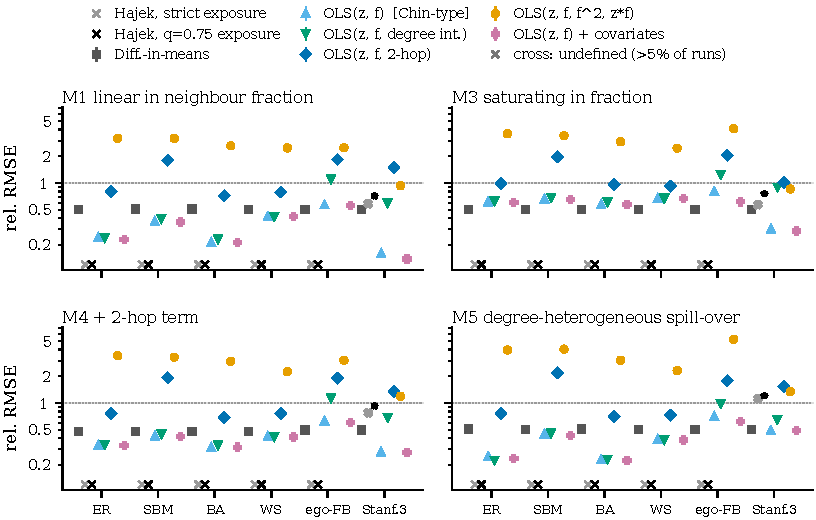
\includegraphics[width=0.99\linewidth]{figA1_headline_bern0.1.pdf}
\caption{As Fig.~\ref{fig:headline}, Bernoulli$(0.1)$.}\label{fig:a1a}
\end{figure}
\begin{figure}[H]\centering
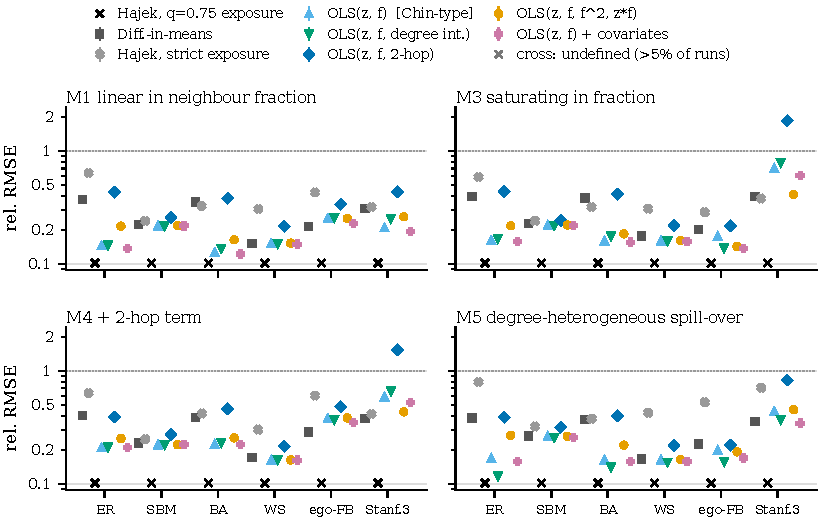
\includegraphics[width=0.99\linewidth]{figA1_headline_cluster0.5.pdf}
\caption{As Fig.~\ref{fig:headline}, graph-cluster randomisation ($p=0.5$).}\label{fig:a1b}
\end{figure}

\paragraph{Seed replication (Fig.~\ref{fig:seed}).}\label{app:seed} A second, independent seed set for the 48 synthetic main-grid cells reproduces the relative RMSE of every estimator.
\begin{figure}[H]\centering
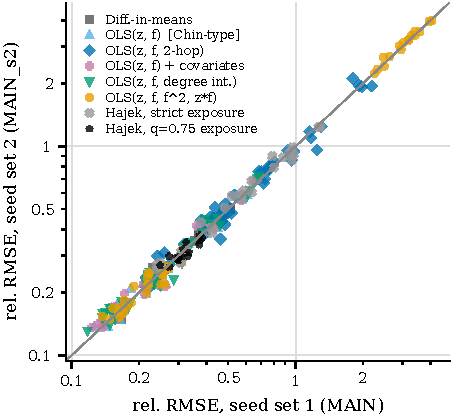
\includegraphics[width=0.55\linewidth]{figA2_seed_replication.pdf}
\caption{Relative RMSE under the first versus the second seed set, synthetic main-grid cells.}\label{fig:seed}
\end{figure}

\paragraph{Bias versus variance and coverage on the main grid (Figs.~\ref{fig:biassd}, \ref{fig:cov-bias}).}
\begin{figure}[H]\centering
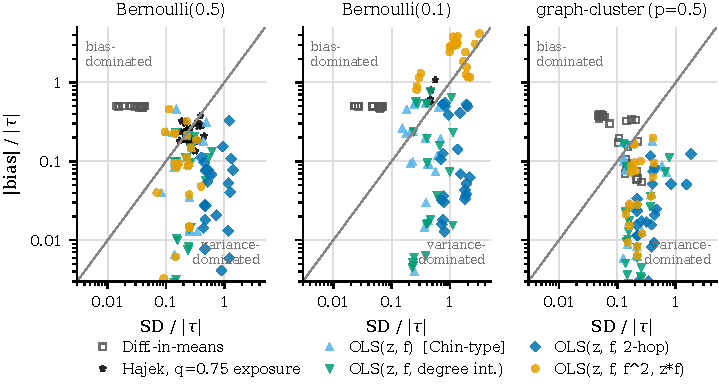
\includegraphics[width=0.87\linewidth]{fig2_bias_sd.pdf}
\caption{$|$Bias$|/|\gate|$ against SD$/|\gate|$ of each estimator, one point per main-grid cell, by design; the diagonal separates bias- from variance-dominated error.}\label{fig:biassd}
\end{figure}
\begin{figure}[H]\centering
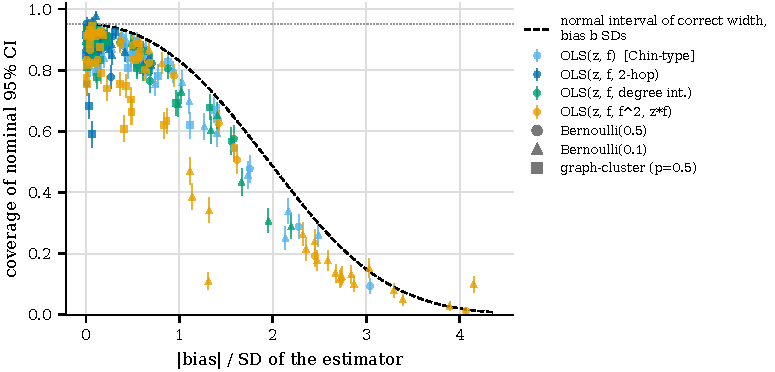
\includegraphics[width=0.94\linewidth]{fig4_coverage.pdf}
\caption{Coverage of the nominal 95\% interval against $|\text{bias}|/\mathrm{SD}$, main grid.}\label{fig:cov-bias}
\end{figure}


\paragraph{Diagnostic, design and graph errors (Figs.~\ref{fig:h7}, \ref{fig:design}, \ref{fig:grapherr}).}
\begin{figure}[H]
\centering
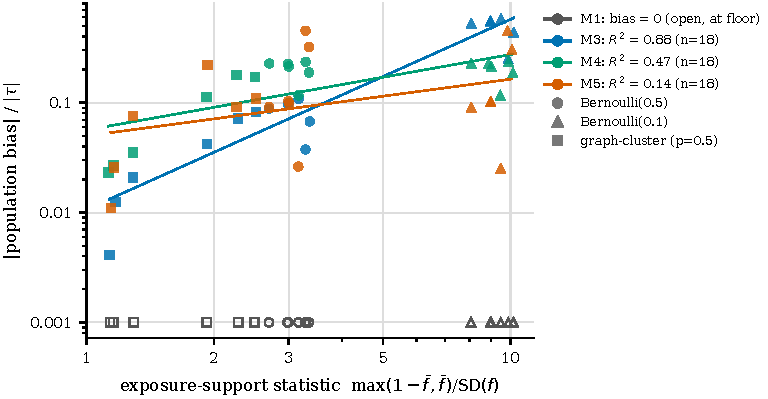
\includegraphics[width=0.93\linewidth]{fig3_h7_diagnostic.pdf}
\caption{Exposure-support statistic against the absolute population bias of OLS$(z,f)$ on the main grid, one point per cell, per-mechanism log--log regression; cells with no bias (M1) are drawn open at the floor.}
\label{fig:h7}
\end{figure}
\begin{figure}[H]
\centering
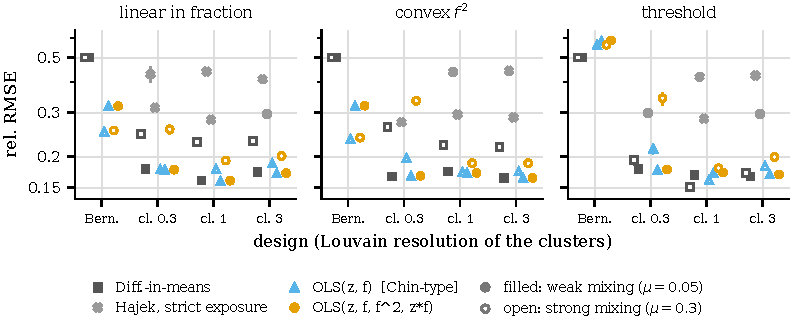
\includegraphics[width=0.96\linewidth]{fig12_design.pdf}
\caption{Bernoulli versus graph-cluster randomisation at three Louvain resolutions, weak (filled) and strong (open) mixing between blocks, for linear, convex and threshold exposure (SBM, $n=4{,}000$, mean degree 20).}
\label{fig:design}
\end{figure}
\begin{figure}[H]
\centering
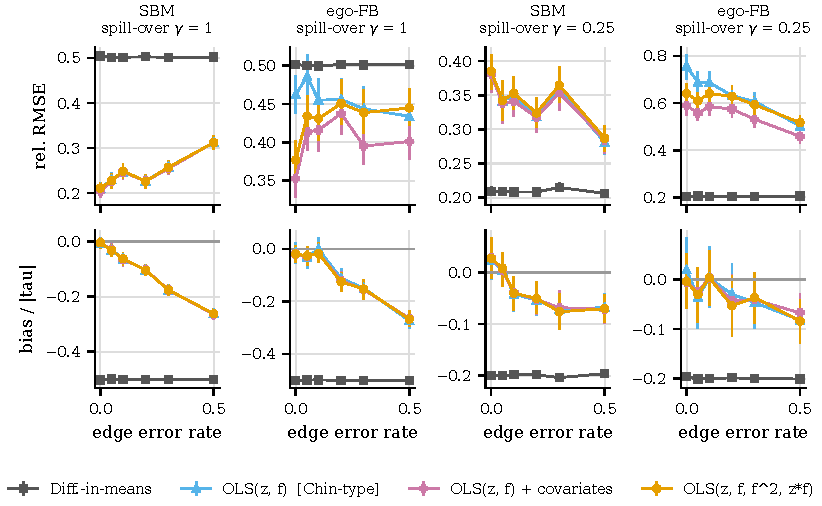
\includegraphics[width=1\linewidth]{fig5_graph_error.pdf}
\caption{Error against the share of edges dropped and re-added in the graph used to build $f$ (8 perturbation draws on the SBM, 12 on ego-Facebook), strong ($\rho=1$) and weak ($\rho=0.25$) interference.}
\label{fig:grapherr}
\end{figure}

\paragraph{Degree and noise (Figs.~\ref{fig:degree}, \ref{fig:noise}).}
\begin{figure}[H]\centering
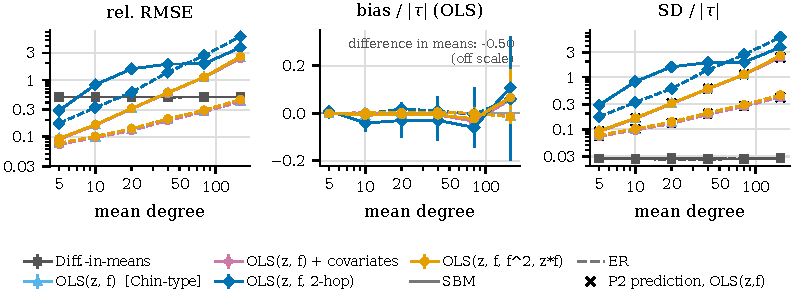
\includegraphics[width=0.96\linewidth]{fig10_degree.pdf}
\caption{Relative RMSE, relative bias and relative SD against mean degree for the Chin-type OLS$(z,f)$, its degree-interaction and quadratic variants and DM, on SBM (solid) and ER (dashed) graphs.}\label{fig:degree}
\end{figure}
\begin{figure}[H]\centering
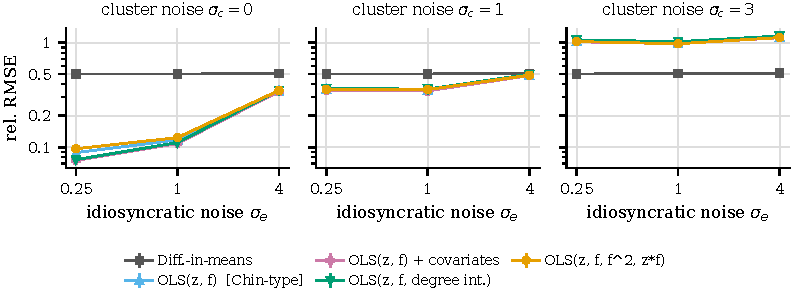
\includegraphics[width=0.96\linewidth]{fig16_noise.pdf}
\caption{Relative RMSE against the idiosyncratic noise SD $\sigma_e$ for community-level baseline SD $\sigma_c=0,1,3$ (SBM; DM grey).}\label{fig:noise}
\end{figure}

\paragraph{Bias and SD against $n$ and $\rho$ (Figs.~\ref{fig:sizeapp}, \ref{fig:gammaapp}).}
\begin{figure}[H]\centering
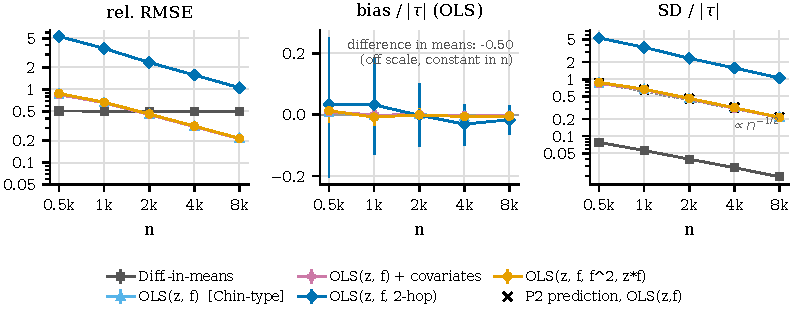
\includegraphics[width=0.96\linewidth]{fig6_size.pdf}
\caption{Bias, SD and relative RMSE against $n$ for the correctly specified linear mechanism (SBM, mean degree 20); the SD of OLS follows the $n^{-1/2}$ reference and the P2 prediction.}\label{fig:sizeapp}
\end{figure}
\begin{figure}[H]\centering
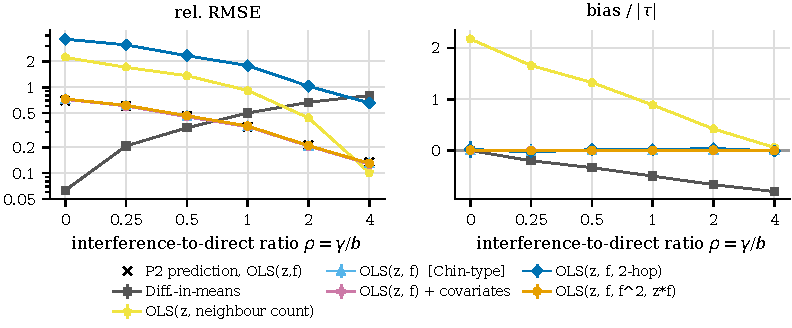
\includegraphics[width=0.96\linewidth]{fig7_gamma.pdf}
\caption{The same against the interference ratio $\rho$ ($n=3{,}000$). OLS on the raw neighbour count is strongly biased, most at $\rho=0$.}\label{fig:gammaapp}
\end{figure}

\paragraph{Feature set versus form of interference (Figs.~\ref{fig:spec}, \ref{fig:specbias}).}
\begin{figure}[H]\centering
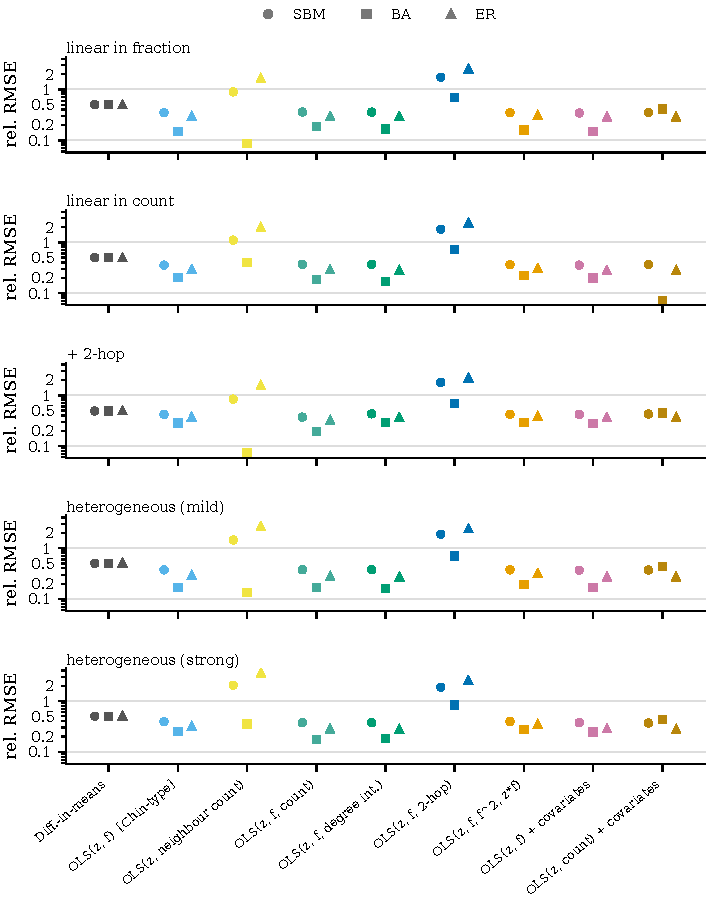
\includegraphics[width=0.86\linewidth]{fig11_specification.pdf}
\caption{Error of feature sets (rows) for different true exposure forms (linear fraction, linear count, two-hop, degree-heterogeneous) on ER, SBM and BA.}\label{fig:spec}
\end{figure}
\begin{figure}[H]\centering
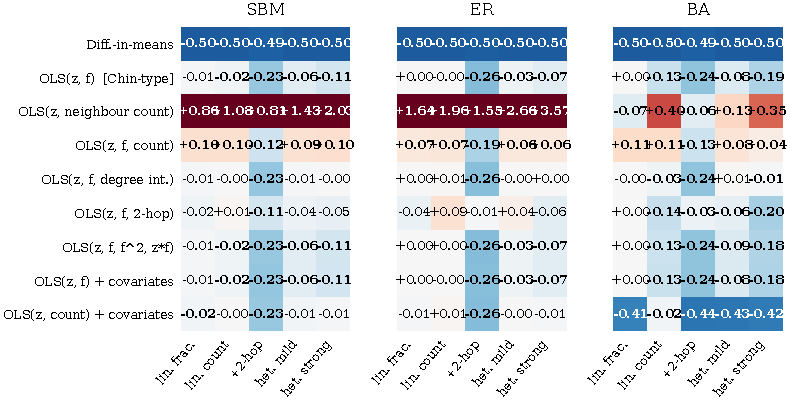
\includegraphics[width=0.96\linewidth]{fig11b_specification_bias.pdf}
\caption{Signed relative bias of the feature sets for each true exposure form (heat map; bold: interval excludes zero). OLS$(z,f)$ is within $\pm0.02$ on SBM and ER for the linear forms and about $-0.25$ under an omitted two-hop term; the degree interaction removes the heterogeneity bias but not the two-hop bias.}\label{fig:specbias}
\end{figure}

\paragraph{Graph families (Fig.~\ref{fig:families}) and observed error against $p$.}
\begin{figure}[H]\centering
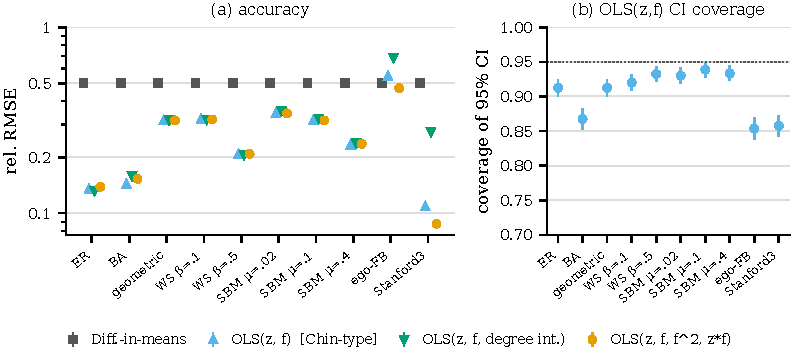
\includegraphics[width=0.96\linewidth]{fig14_graph_families.pdf}
\caption{Ten graph families (synthetic at $n=4{,}000$, mean degree 20, and the two Facebook graphs): (a) relative RMSE of DM and of OLS variants; (b) coverage of the 95\% interval for OLS$(z,f)$.}\label{fig:families}
\end{figure}
\begin{figure}[H]\centering
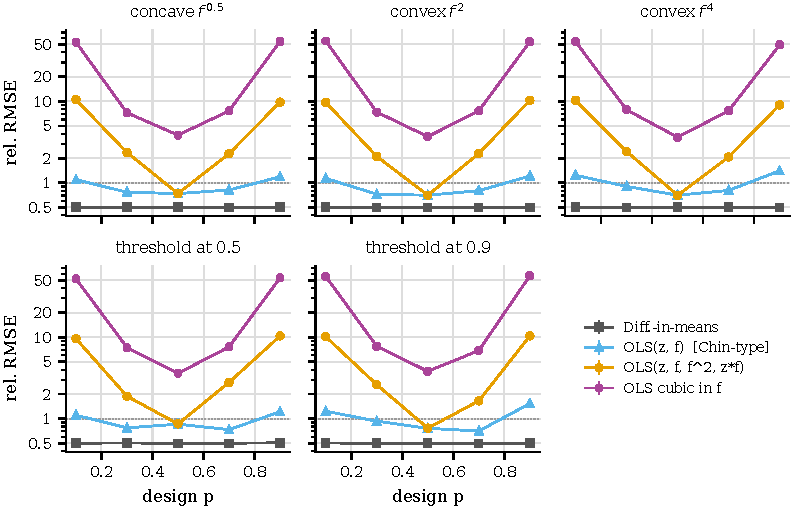
\includegraphics[width=0.96\linewidth]{fig9_curvature_rmse.pdf}
\caption{Observed relative RMSE against the design $p$ for the responses of Fig.~\ref{fig:curv} (degree 40); the quadratic model pays in variance what it gains in bias.}\label{fig:curvobs}
\end{figure}
\begin{figure}[H]\centering
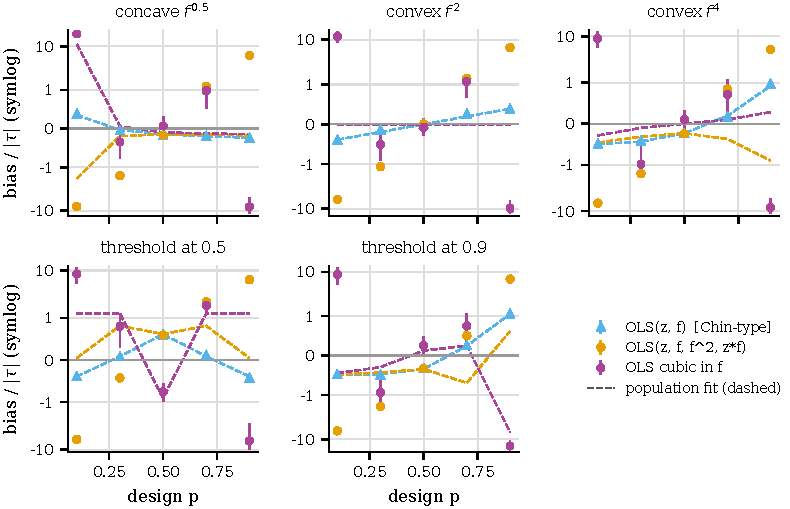
\includegraphics[width=0.96\linewidth]{fig9b_curvature_bias_observed.pdf}
\caption{Observed against population-fit bias (degree 40). For OLS$(z,f)$ the two agree; for the quadratic and cubic models the observed bias is far larger at $p=0.1,0.9$, i.e.\ they err by more than their approximation error (we did not test the cause).}\label{fig:curvbiasobs}
\end{figure}

\paragraph{Theory checks (Fig.~\ref{fig:theory}).}
\begin{figure}[H]\centering
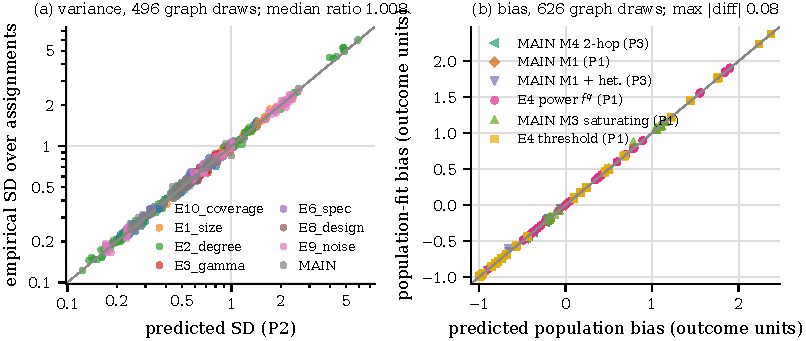
\includegraphics[width=0.98\linewidth]{fig17_theory_check.pdf}
\caption{(a) Predicted (P2) against empirical SD of OLS$(z,f)$ over \TheoryVarN{} graph draws from several experiments; (b) predicted (P1/P3) against noise-free population bias over \TheoryBiasN{} draws; both relative to $|\gate|$, diagonal is exact agreement.}\label{fig:theory}
\end{figure}
